% Appendix D -- Figure 4 and the tail-variance argument behind Section 6's
% recommendation of the normalised construction over the group-conditional one.
% One subsection would be redundant with the section itself, so both labels sit
% on the section: `sec:appendix_conformal_results` is what Section 6 \refs.
\section{Conformal Coverage Diagnostics and Severe-Tail Analysis}
\label{app:conformal}
\label{sec:appendix_conformal_results}

\begin{figure*}[tb]
  \centering
  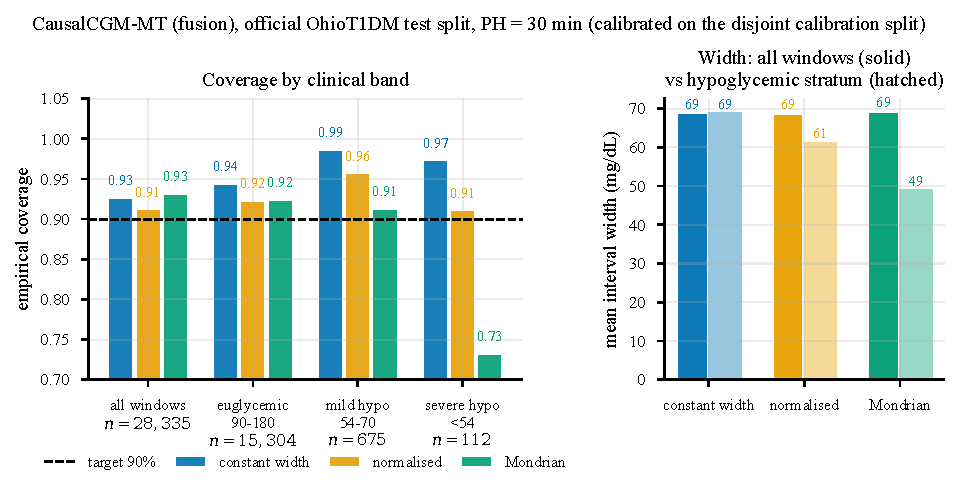
\includegraphics[width=\textwidth]{fig4_conformal_coverage.pdf}
  \caption{Empirical coverage by clinical band and mean interval width for three
  conformal constructions on identical predictions and rows, $\PH = 30$~min,
  $\alpha = \NumAlpha$ (calibrated on the disjoint calibration split, never on
  the validation rows that selected the checkpoint). Mondrian equalises coverage across zones; on this model
  that means \emph{narrowing} the hypoglycemic interval rather than widening it.}
  \label{fig:coverage}
\end{figure*}

A four-zone taxonomy splitting $<54$ out is the obvious response, and at this
sample size it is statistically unavailable rather than merely inconvenient. Two
conditions bind. The first is feasibility: a stratum can certify level $\alpha$
only once it holds $\lceil (1-\alpha)/\alpha \rceil$ calibration points, below
which the required order statistic does not exist and our
\texttt{conformal\_quantile} returns $+\infty$ by construction rather than
falling back to the sample maximum. The second, and the binding one here, is
variance. Conditional on the calibration draw, split-conformal coverage is
$\mathrm{Beta}(n + 1 - \ell,\, \ell)$ with $\ell = \lfloor (n+1)\alpha \rfloor$,
so its standard deviation is of order $\sqrt{\alpha(1-\alpha)/n}$. The $<54$ test cell
holds $\NumSevereN$ windows, so coverage measured in it has a sampling standard
deviation of the same order, near $\NumSevereCovSDPts$ percentage points, before the interval half-width (itself an extreme order
statistic of a small sample) contributes its own dispersion. A dedicated
stratum would therefore certify a conditional guarantee whose realised coverage
moves, from calibration draw to calibration draw, by an amount comparable to the
miscoverage it was introduced to repair. The estimator's variance would dominate
the effect it estimates, which is a worse instrument than the pooled quantile it
replaced, not a better one.

The alternative is to leave the quantile pooled and make the \emph{width}
locally adaptive, which is what the normalised construction does: it scales one
calibration quantile by $\sigma$, the mean absolute glucose change over the last
30 minutes of the input window (\texttt{rate\_of\_change\_difficulty}). Nothing
in $\sigma$ is fitted; it is a fixed function of the history, so it adds no
estimation variance of its own, but it also carries no guarantee that it tracks
difficulty in the severe tail.

The measurements do not separate split and normalised conformal in that cell. Normalised
conformal reaches $\NumNormSevereCov$ coverage below 54~mg/dL, against
$\NumSplitSevereCov$ for split conformal and $\NumMondrianSevereCov$ for
Mondrian, at a mean width of $\NumNormWidth$~mg/dL against $\NumSplitWidth$, and
holds the hypoglycemic band at $\NumNormHypoCov$ against split conformal's
$\NumSplitHypoCov$. Mondrian's narrower hypoglycemic width
($\NumMondrianHypoWidth$~mg/dL, against $\NumNormHypoWidth$ for normalised and
$\NumSplitHypoWidth$ for split conformal) is bought with the
severe-tail undercoverage above. Because the severe cell is small and
autocorrelated, we report the spread of each construction's coverage there
across block-bootstrap resamples of the calibration split (resampling
subject-days, recalibrating, and rescoring the fixed test windows) rather than a
single realisation, and make no recommendation that this spread does not
support.

\paragraph{Which regime one is in.}
We stress that these are properties of \emph{this} model on \emph{this} split.
On a patient-disjoint arm with a weaker model we observe the more commonly
reported pattern instead: severe undercoverage below 70 that stratification
substantially repairs. Which regime one is in should be measured, and we ship
\texttt{scripts/verify\_mondrian\_coverage.py} for that purpose rather than
asserting a figure in prose.
